\documentclass[dvipdfmx]{standalone}
\usepackage{tikz}
\usetikzlibrary{calc}
%
\begin{document}
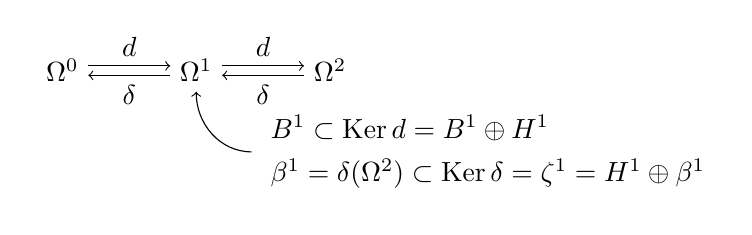
\begin{tikzpicture}[scale=1]
    \matrix[column sep = 3em]{
        \node(o0){$\Omega^0$}; & \node(o1){$\Omega^1$}; & \node(o2){$\Omega^2$}; \\
    };

    \coordinate (pp) at (0,0.06);

    \draw[->]($(o0.east)+(pp)$)--node[midway, above]{$d$}($(o1.west)+(pp)$);
    \draw[<-]($(o0.east)-(pp)$)--node[midway, below]{$\delta$}($(o1.west)-(pp)$);

    \draw[->]($(o1.east)+(pp)$)--node[midway, above]{$d$}($(o2.west)+(pp)$);
    \draw[<-]($(o1.east)-(pp)$)--node[midway, below]{$\delta$}($(o2.west)-(pp)$);

    \begin{scope}[xshift=2em, yshift=-4em]
        \matrix(T)[anchor=base west]{
            \node{$B^1 \subset \mathop{\mathrm{Ker}} d = B^1 \oplus H^1$}; \\
            \node{$\beta^1 = \delta(\Omega^2) \subset \mathop{\mathrm{Ker}} \delta = \zeta^1 = H^1 \oplus \beta^1$};\\
        };
    \end{scope}

    \draw[->](T.west)to[out=180, in=-90](o1.south);

\end{tikzpicture}
\end{document}
